En esta sección se entrará a describir con total detalle el contenido técnico de la aplicación. Partiendo desde un analisis de requisitos funcionales
hasta no funcionales, pasando por las tecnologías usadas para la implemetación de estos. 

\section{Tecnologias Empleadas}

\subsection{SpringBoot}
Spring Boot es un marco de trabajo Java que simplifica el desarrollo de aplicaciones web al eliminar la 
complejidad de la configuración manual. Ofrece configuración automática, empaquetado de aplicaciones independientes y un inicio rápido integrado, 
lo que permite a los desarrolladores crear aplicaciones de manera más rápida y eficiente, centrándose en la lógica de negocio en lugar de la configuración. 
Genial para el desarrollo de aplicaciones \textit{CRUD}\footnote{\textit{CRUD} es un acrónimo en inglés que se refiere a las operaciones 
básicas de manipulación de datos en aplicaciones informáticas: Create (Crear), Read (Leer), Update (Actualizar) y Delete (Eliminar).}.
\subsection{Maven}
Maven es una herramienta de gestión de proyectos Java que simplifica la estructuración, gestión de dependencias y automatización de la construcción. 
Permite definir dependencias en un archivo de configuración (pom.xml), ejecutar fases de construcción estandarizadas y gestionar repositorios 
centralizados de bibliotecas. Es ampliamente utilizado en el desarrollo Java por su integración con IDEs y su capacidad para proyectos multiproyecto, es decir,
permite la gestión de múltiples proyectos en un solo repositorio, lo que facilita la colaboración entre desarrolladores y la gestión.
\subsection{Vue.js}
Vue.js es un popular marco de trabajo de código abierto para construir interfaces de usuario interactivas en aplicaciones web de una sola página. 
Se destaca por su enfoque centrado en el componente, su sintaxis declarativa y su eficiente sistema de reactividad. Vue.js facilita la construcción 
de aplicaciones web complejas al fomentar la reutilización de componentes y ofrecer herramientas integradas para la manipulación del DOM y la gestión 
del estado de la aplicación.

\subsection{MySQL}
MySQL es un sistema de gestión de bases de datos relacional de código abierto ampliamente utilizado en el desarrollo de 
aplicaciones web y empresariales. Destaca por su escalabilidad, rendimiento, fiabilidad y facilidad de uso. Ofrece opciones 
sólidas de seguridad y es compatible con una variedad de plataformas y lenguajes de programación. MySQL es una herramienta poderosa 
para gestionar eficientemente grandes volúmenes de datos y garantizar la integridad y disponibilidad de la información.

\subsection{IntelliJ}
IntelliJ IDEA es un entorno de desarrollo integrado (IDE) altamente productivo desarrollado por JetBrains. 
Diseñado para diversas tecnologías, ofrece una interfaz de usuario intuitiva y funciones avanzadas que mejoran la 
productividad del desarrollador. Con soporte para múltiples lenguajes y marcos de trabajo, integración con herramientas de desarrollo y 
características colaborativas, IntelliJ IDEA es una opción popular para el desarrollo de software en Java y otros lenguajes.

\subsection{VSCode}
Visual Studio Code (VSCode) es un IDE popular desarrollado por Microsoft, conocido por su versatilidad, rendimiento y comunidad activa.
 Ofrece características avanzadas y extensiones para diferentes lenguajes de programación. Es altamente personalizable y cuenta con una 
 amplia documentación disponible en su sitio web oficial.

\subsection{AWS S3}
AWS S3 es un servicio de almacenamiento en la nube ofrecido por Amazon Web Services. Destaca por su escalabilidad, durabilidad, seguridad y 
facilidad de uso. Permite almacenar grandes cantidades de datos de forma segura y acceder a ellos de manera eficiente a través de una interfaz 
intuitiva y una API robusta. Con una estructura de precios flexible, AWS S3 es una opción atractiva para empresas que buscan una solución de 
almacenamiento en la nube rentable y confiable.

\subsection{AWS EC2}
AWS EC2 es un servicio de cómputo en la nube proporcionado por Amazon Web Services. Destaca por su escalabilidad, flexibilidad y seguridad. 
Permite a los usuarios alquilar capacidad informática según sus necesidades, con opciones de pago por uso. Es fácil de usar y ofrece una variedad 
de opciones de implementación. En resumen, EC2 es una solución eficiente y confiable para ejecutar aplicaciones y cargas de trabajo en la nube.

\subsection{Docker}
Docker es una plataforma de código abierto que permite crear, implementar y ejecutar aplicaciones en contenedores. Destaca por su portabilidad, 
eficiencia y facilidad de uso. Con la tecnología de contenedores, Docker ofrece aislamiento de aplicaciones y escalabilidad, lo que simplifica el 
desarrollo y la administración de aplicaciones en diferentes entornos. En resumen, Docker es una herramienta fundamental para la creación y gestión 
eficiente de aplicaciones modernas.

\newpage
\section{Resumen de las tecnologias}
La Tabla \ref{tabla:tecnologias_usos} recoge un resumen de las tecnologías empleadas para el desarrollo de Enterprise Event Solutions
\begin{table}[h]
\begin{tabular}{ p{3cm} l  }

    \hline
    Tecnologia& Uso \\
    \hline
    SpringBoot   & Framework \\
    Maven &   Framework \\
    Vue.js & Framework  \\
    MySQL    & Tecnologia de BD \\
    IntelliJ&   Entorno de Desarrollo  \\
    VSCode& Entorno de Desarrollo \\
    AWS S3& Tecnologia de de BD en la nube  \\
    AWS EC2& Servidor web en la nube  \\
    Docker& Crecion de imagenes comprimidas para despliegue  \\
    \hline
   \end{tabular}
   \caption{Tecnologías y sus usos correspondientes}
   \label{tabla:tecnologias_usos}
\end{table}
\newpage
\section{Arquitectura}
\textbf{Enterprise Event Solutions} es una aplicación \textbf{Fullstack} creada siguiendo un patrón de diseño MVC. A continuación, se muestra un plano general
que será desglosado:  CAMBIAR DIAGRAMA !!!!1 AÑADIR SEGURIDAD 

\section*{Arquitectura General}
\begin{figure}[h]
    \centering
    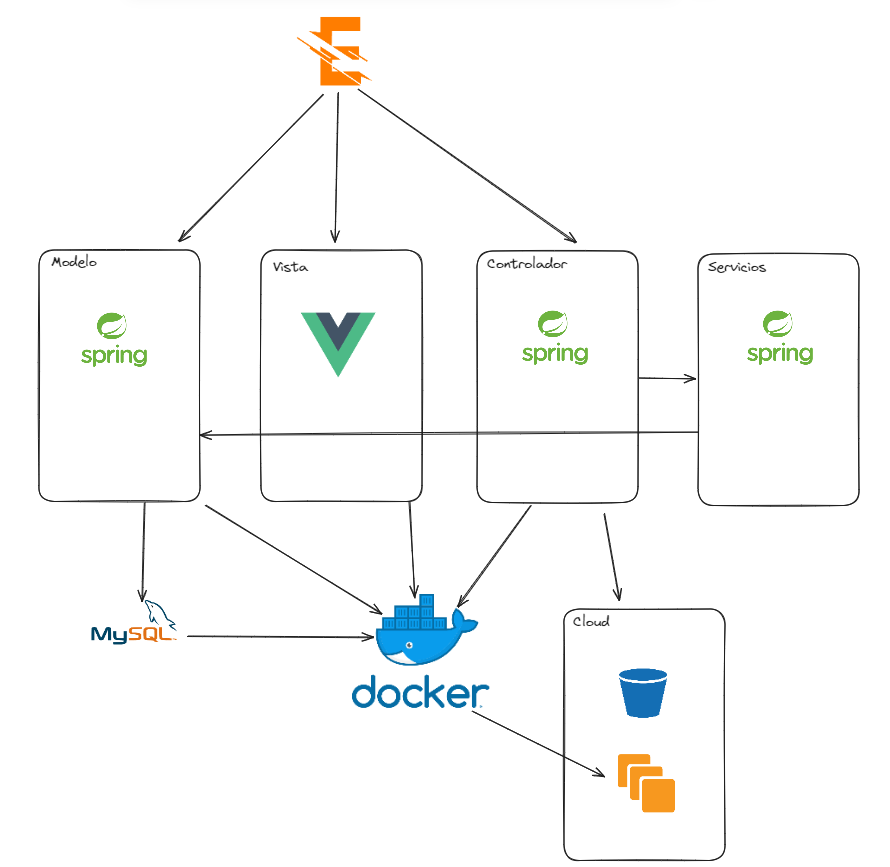
\includegraphics[width=0.8\textwidth]{Arquitectura.png} 
    \caption{Diagrama de Arquitectura de EVS}
    \label{fig:mvc_architecture}
\end{figure}
\newpage

\section*{Backend (Modelo y Controlador)}

\begin{itemize}
    \item \textbf{Tecnología}: \textbf{SpringBoot}
    \item \textbf{Descripción}: Utilizado por su gran versatilidad para manejar la lógica de negocio y control de la aplicación. Gracias a esto, el frontend
    de la aplicación se sirve directamente desde el Servidor de Apache proporcionado por spring, es decir, tengo empaquetado el tanto el back como el front en la misma ip
    y en el mismo puerto.
\end{itemize}

\section*{Frontend (Vista)}

\begin{itemize}
    \item \textbf{Tecnología}: \textbf{Vue.js}
    \item \textbf{Descripción}: Seleccionado para explorar otras tecnologías y facilitar la creación de una interfaz de usuario interactiva.
\end{itemize}

\section*{Tecnologías Complementarias}

\begin{itemize}
    \item \textbf{AWS EC2}: 
    \begin{itemize}
        \item \textbf{Descripción}: Instancia EC2 para desplegar la aplicación, ofreciendo un entorno robusto y escalable.
    \end{itemize}
    \item \textbf{AWS S3}:
    \begin{itemize}
        \item \textbf{Descripción}: Bucket S3 para almacenar imágenes, reduciendo la carga de trabajo en la base de datos.
    \end{itemize}
    \item \textbf{MySQL}:
    \begin{itemize}
        \item \textbf{Descripción}: Base de datos utilizada para gestionar los datos de la aplicación de manera eficiente.
    \end{itemize}
\end{itemize}

\textbf{Enterprise Event Solutions} combina las fortalezas de \textbf{SpringBoot} y \textbf{Vue.js} en un patrón MVC para ofrecer una solución robusta y 
escalable. Con el soporte de \textbf{AWS} y \textbf{MySQL}, la aplicación está preparada para manejar grandes volúmenes de datos y ofrecer una experiencia 
de usuario fluida.


Cada uno de los componentes definidos en la Imagen \ref{fig:mvc_architecture} será desglosado en las próximas secciones para explicar detalladamente el contenido de 
la aplicación.

\subsection{Modelo}
La persistencia en Enterprise Event Solutions se sustenta en una serie de Entidades almacenadas en una base de datos con la que los servicios interactuan mediante
las interfaces proporcionadas por JPA \ref{sec:jpa}. Es el pilar fundamental en el que se sustenta el modelo de negocio de la aplicación.
\begin{figure}[h]
    \centering
    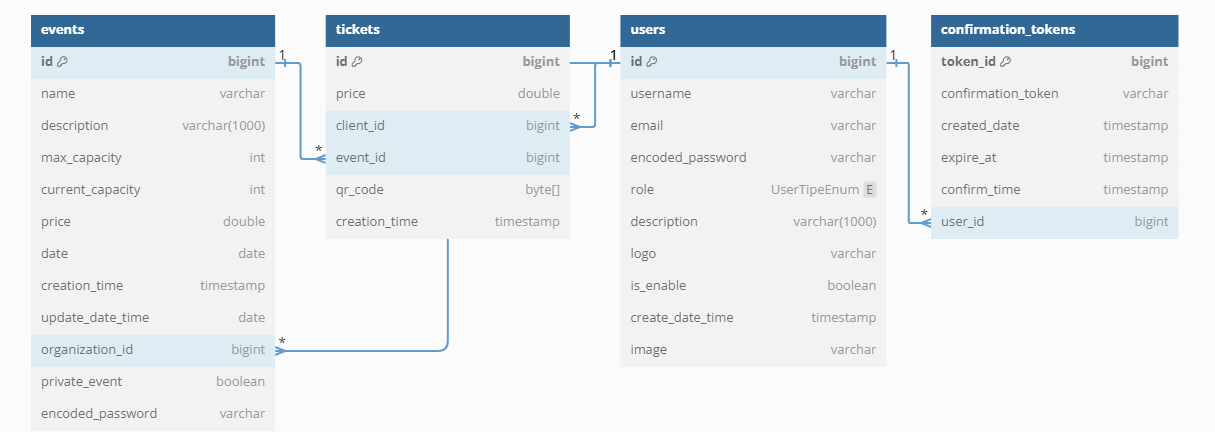
\includegraphics[width=1.2\textwidth]{EVSdiagra.png} 
    \caption{Modelo E-R de la BD}
    \label{fig:diagramaBD}
\end{figure}

\subsubsection{JPA}
\label{sec:jpa}

JPA (Java Persistence API) es una especificación de Java que facilita la gestión de la persistencia de datos en aplicaciones Java.
En Spring, se usa para simplificar las operaciones CRUD y el manejo de relaciones entre entidades, permitiendo trabajar con objetos en lugar de SQL. 
Spring Data JPA integra JPA en el ecosistema Spring, proporcionando repositorios predefinidos para operaciones de base de datos comunes.

A continuación se muestra un fragmento de código de Spring Data JPA en Java:
\myjavastyle
\begin{lstlisting}[language=Java, caption=Ejemplo de Repositorio en Spring Data JPA]
@Repository
public interface UserRepository extends JpaRepository<User,Long> {
    public Optional<User> findByEmail(String email);
    public List<User> findAllByRole(UserTipeEnum type);
    public Optional<User> findByUsername(String username);
}
\end{lstlisting}

Como se puede observar, gracias a la gran potencia de Spring y de JPA, simplemente con crear una interfaz con metodos que creemos que vamos a necesitar en 
nuestros servicios, y sin la necesidad de añadir @Querys, podemos hacer consultas sobre la base de datos.

Pero también podemos hacer nuestras propias Querys sobre la base de datos:
\myjavastyle
\begin{lstlisting}[language=Java, caption=Ejemplo de Query  en Spring Data JPA]
    @Transactional
    @Modifying
    @Query("UPDATE Event e SET e.current_capacity = e.current_capacity + 1 WHERE e.id = :id AND e.current_capacity + 1  <= e.max_capacity")
    public int incrementCurrentCapacity(@Param("id") Long id);
\end{lstlisting}

\subsection{Contolador}
La creación de controladores me ha permitido gestionar un sistema de endpoints que sirve como la interfaz principal 
para la comunicación entre el cliente y el servidor. Estos controladores se encargan de recibir las solicitudes HTTPS de delegar el procesamiento a 
los servicios correspondientes. Los servicios encapsulan la lógica de negocio y se comunican con los repositorios JPA para acceder a los datos de la 
base de datos de manera eficiente. Además, para garantizar la seguridad, se utiliza JWT (JSON Web Tokens), que permite la autenticación y autorización 
de los usuarios. Los tokens JWT se generan tras un inicio de sesión exitoso y se utilizan para proteger los endpoints, asegurando que solo los usuarios 
autenticados puedan acceder a recursos específicos. Este enfoque no solo organiza el código de manera modular y mantenible, sino que también proporciona 
una robusta capa de seguridad para la API.
\begin{figure}[h]
    \centering
    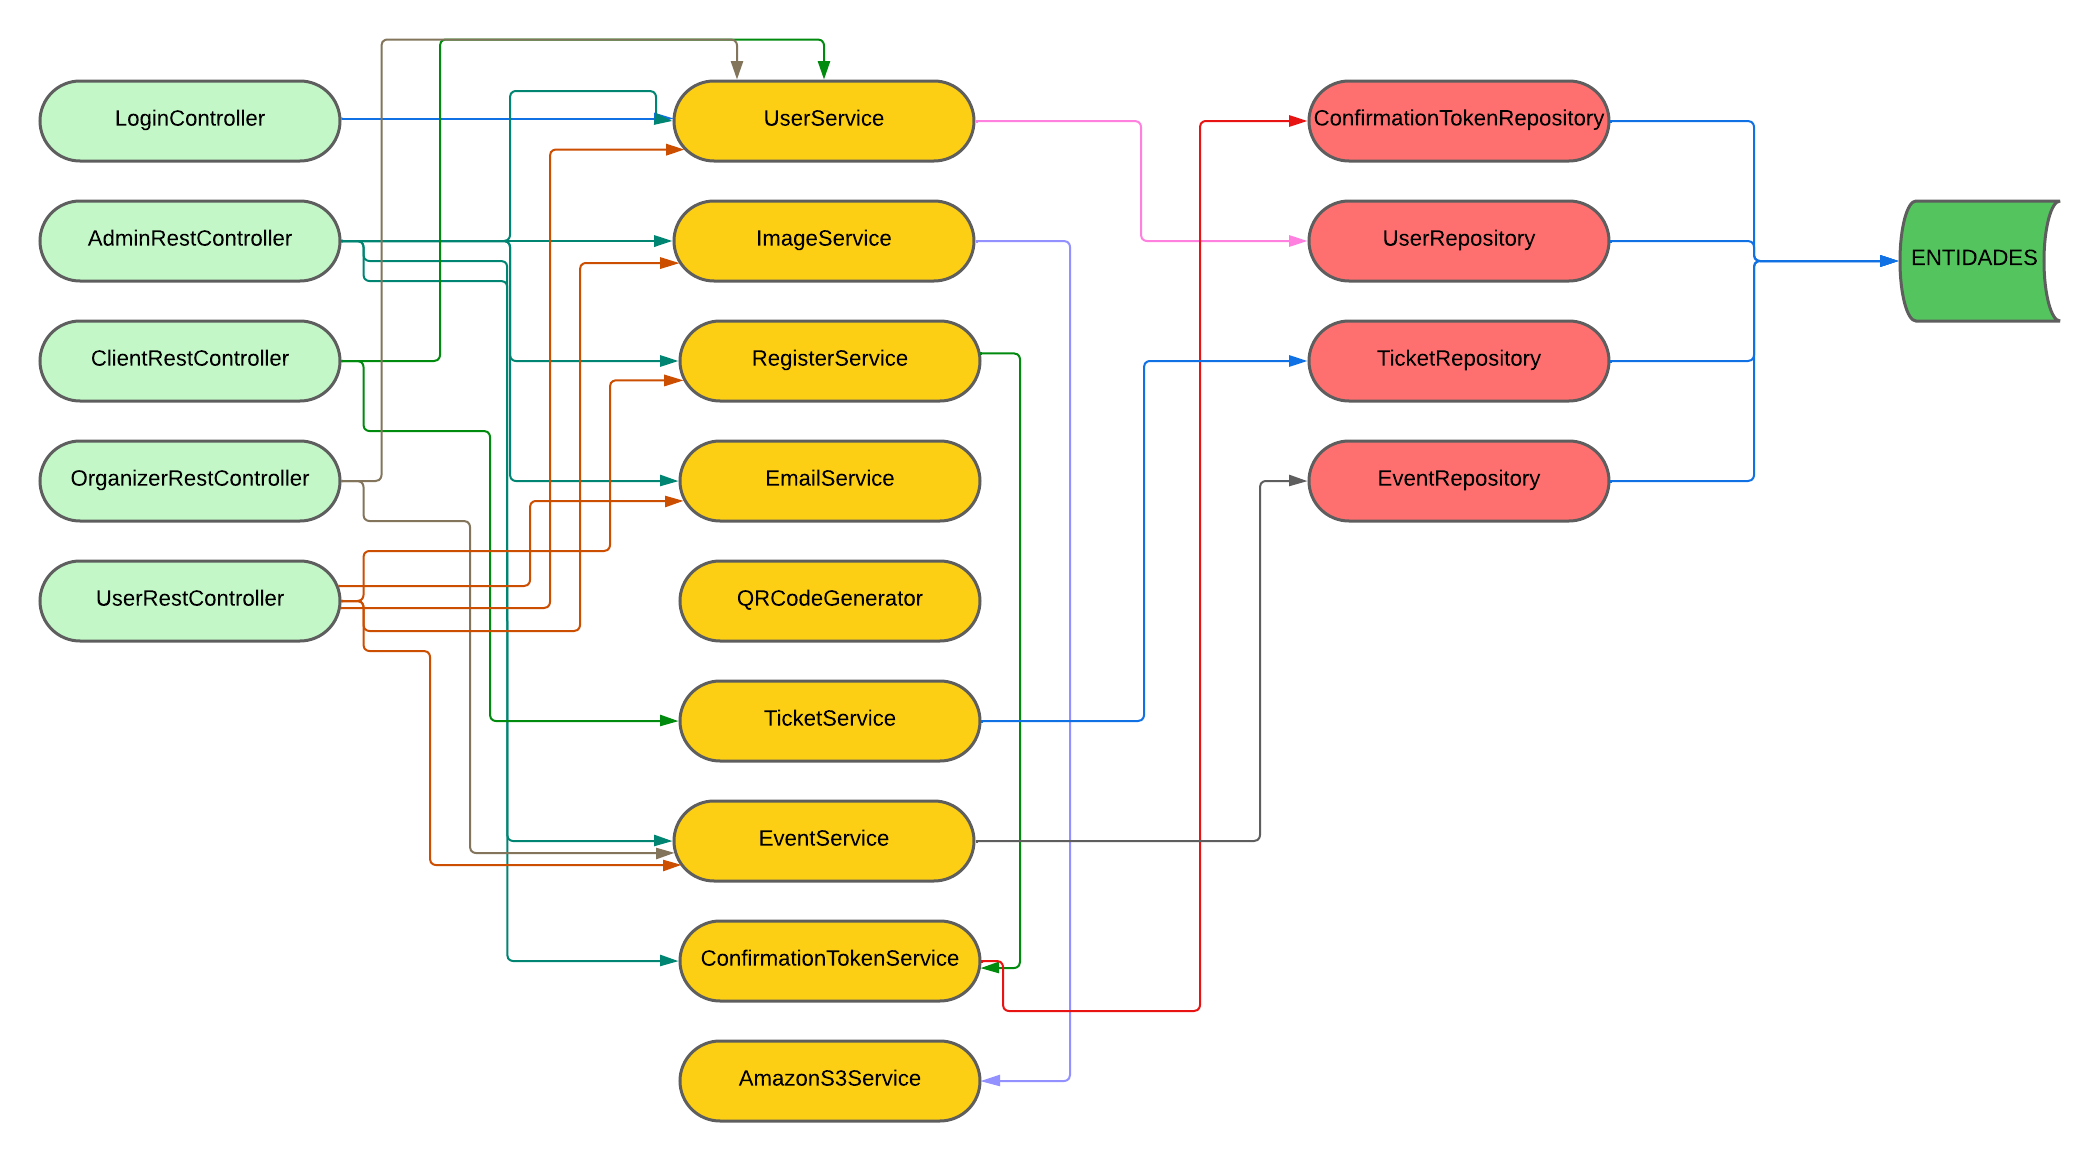
\includegraphics[width=1\textwidth]{DiagramaClases.png} 
    \caption{Diagrama de Clases de EVS}
    \label{fig:class_architecture}
\end{figure}

Además he implementado otras configuraciones para añadir una capa extra de seguridad a la aplicación como configuración CSRFH y Cors para limitar las url 
que pueden hacer uso de los endpoints de mi app. Por supuesto he creado las configuraciones necesarias para manejar las tecnologias externas como S3, dentro de 
EVS.
\begin{figure}[h]
    \centering
    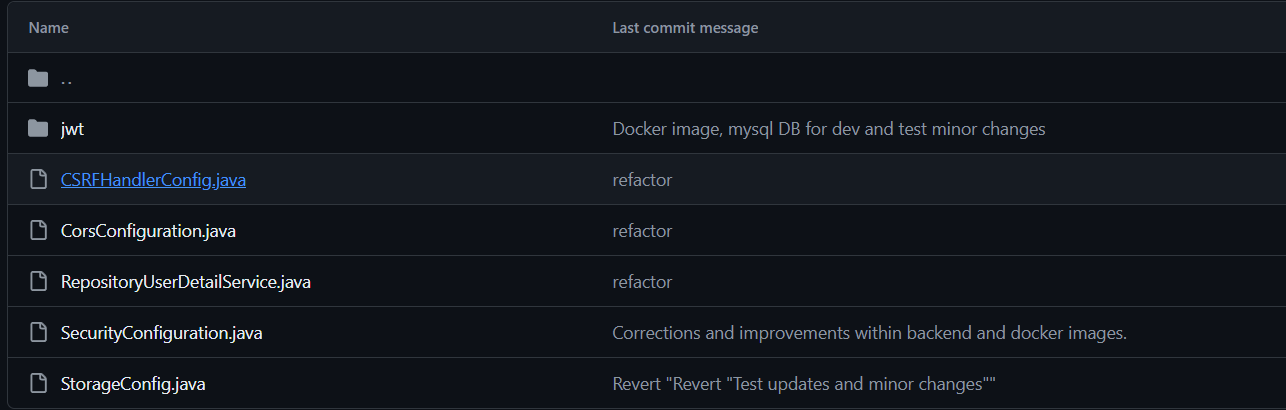
\includegraphics[width=1\textwidth]{security.png} 
    \caption{Seguridad del backend}
    \label{fig:securityClasses}
\end{figure}

\subsection{Vista}
El frontend de Enterprise Event Solution ha sido implementado en Vue.js. Especificamente en Vue3, que trae consigo algunos cambios con respecto a su versión
anterior Vue2. La utilización de este framework me ha permitido añadir tanto bibliotecas de componentes y gráficos (Bootstrap5 y Chart.js respectivamente)
como relaciones entre los diferentes componentes basado en "props", permitiendo de esta manera diferentes comportamientos del componente dependiendo de
que valores se le pasen en el componente padre.

Un ejemplo del uso de estas props sería:
\myvuestyle
\begin{lstlisting}[language=HTML, caption=Ejemplo del Padre, label=lst:padre]
    <event_cards
    :evento="evento"
    :is-org="false"
    >
    </event_cards>
\end{lstlisting}
\myvuestyle
\begin{lstlisting}[language=HTML, caption=Ejemplo del Hijo, label=lst:hijo]
    <script lang="ts">
    import {EventService} from "../services/event.service";
    import { useRouter } from "vue-router";
    import { Event } from "../models/Event";
    import { computed, ref } from "vue";
    export  default {
        name: "event_cards",
        props:{
          evento: Object as ()=> Event,
          isOrg: Boolean,
        },
    }
\end{lstlisting}

En el código \ref{lst:padre}, se observa que se inserta en el template un componente con la información del evento. Por otro lado, en el código 
\ref{lst:hijo}, se manejan estos valores que hemos pasado desde el componente padre. En este fragmento, si se le pasa \texttt{true} en la variable 
\texttt{is-org}, el componente tendrá un comportamiento diferente a si se le pasa \texttt{false}. Ademas en la variable \texttt{evento} le pasamos la información
del evento para garantizar la reactividad de los componetes de forma individual. De esta forma trabajamos con módulos y no con un elemento.